\documentclass[journal]{IEEEtran}

\usepackage{amsmath,amssymb,amsfonts}
\usepackage{algorithmic}
\usepackage{algorithm}
\usepackage{float}
\usepackage{graphicx}
\usepackage{textcomp}
\usepackage{xcolor}
\usepackage{booktabs}
\usepackage{multirow}
\usepackage{url}
\usepackage{hyperref}
\usepackage{cite}
\usepackage{array}
\usepackage{makecell}

\newcommand{\sysname}{TRAP}
\newcommand{\etal}{\textit{et al.}}
\newcommand{\eg}{\textit{e.g.}}
\newcommand{\ie}{\textit{i.e.}}

\begin{document}

\title{Robust Federated Learning for Credit Card Identity Fraud Detection}

\author{%
  \IEEEauthorblockN{Anonymous Authors}
  \IEEEauthorblockA{(Under Review --- IEEE Transactions on Information Forensics and Security)}
}

\maketitle

% ─────────────────────────────────────────────────────────────────────────────
\begin{abstract}
Credit card fraud causes billions of dollars in annual losses worldwide.
While centralized machine learning models have proven effective at detecting
fraudulent patterns, financial institutions are constrained from sharing raw
transaction data by regulatory frameworks such as GDPR and PSD2.
Federated learning (FL) offers a compelling alternative, enabling banks to
collaboratively train a shared fraud detection model without exchanging raw
records. However, this collaborative setting introduces a critical
vulnerability: a financially-motivated adversary controlling a compromised
bank node can poison the shared model to specifically evade detection of
their own fraud patterns. Crucially, standard Byzantine-robust aggregators
are \emph{stateless}---they evaluate each round independently---rendering
them blind to adaptive attackers who schedule their poisoning across rounds.
In this paper, we propose \sysname{} (Temporal Reputation-Aware Poisoning
defense), a gated cascade defense framework that combines norm/cosine
filtering (Layer~1), Leave-One-Out spectral anomaly detection (Layer~2),
and dual-channel CUSUM temporal consistency tracking (Layer~3), coordinated
by an adaptive threshold controller and an EWMA reputation system.
We evaluate \sysname{} on the IEEE-CIS Credit Card Fraud Detection
dataset~\cite{kaggle2019ieeecis} under a realistic Dirichlet non-IID
cross-silo split with 10 clients and 50 communication rounds, directly
comparing against FedAvg~\cite{mcmahan2017fedavg} and
Krum~\cite{blanchard2017krum} with full AUC/F1/Precision/Recall metrics.
Across three attack classes at adversary ratios of 10\%, 20\%, and 40\%,
\sysname{} achieves the highest F1-Score in 8 of 10 scenarios and avoids
the all-benign collapse mode (Recall=0) that afflicts FedAvg under
Sign-Flip attacks and Krum under LabelFlip at 40\%.
A 12-run ablation study demonstrates that all three layers are necessary.
\end{abstract}

\begin{IEEEkeywords}
Federated learning, fraud detection, Byzantine robustness, model poisoning,
credit card fraud, temporal CUSUM, spectral anomaly detection,
adversarial machine learning
\end{IEEEkeywords}

% ─────────────────────────────────────────────────────────────────────────────
\section{Introduction}
\IEEEPARstart{C}{redit} card fraud inflicts enormous financial damage on
banks and consumers alike, with global losses exceeding \$30 billion
annually~\cite{farrukh2025blockchain}. Traditional fraud detection systems
operate in isolation: each financial institution trains predictive models
solely on its own proprietary transaction data, inherently missing
cross-institutional fraud patterns. Regulatory frameworks such as GDPR and
PSD2 strictly restrict raw data sharing, creating a fundamental tension
between privacy preservation and detection efficacy.

Federated learning (FL) resolves this tension by enabling banks to
collaboratively train a shared predictive model without ever exchanging
raw transaction data~\cite{mcmahan2017fedavg}. In the cross-silo FL
setting, participating banks (clients) train local models and transmit
only model parameter updates to a central aggregation
server~\cite{kairouz2021advances}. Recent studies have demonstrated
the viability of FL for credit card fraud detection~\cite{yang2019ffd,abdulsalam2024fl}.

However, a financially-motivated adversary controlling a compromised bank
node has a direct economic incentive to corrupt the shared model: to
suppress detection of their own fraud patterns while maintaining high
accuracy on legitimate transactions to avoid raising
alarms~\cite{bhagoji2019analyzing,bagdasaryan2018backdoor}. This
targeted, incentive-driven evasion poisoning has a key distinguishing
property: \emph{stateless} per-round defenses are inadequate. Standard
robust aggregators such as Krum~\cite{blanchard2017krum} and Trimmed
Mean~\cite{yin2018byzantine} evaluate each round independently. An
adversary that behaves honestly for three rounds, attacks on the fourth,
and pauses on the fifth can evade any per-round static defense. Our
empirical evaluation confirms this: unprotected FedAvg collapses to
Recall=0 (all-benign prediction) under Sign-Flip attacks at 20--40\%
adversary ratio, while Krum catastrophically fails under LabelFlip at 40\%
(AUC=0.413, Recall=0.920 with Precision=0.034—all-fraud prediction).

In this paper, we propose the Temporal Reputation-Aware Poisoning
(\sysname{}) defense framework. Our contributions are:
\begin{enumerate}
  \item A \textbf{three-layer gated cascade} defense (norm/cosine
        filtering, Leave-One-Out spectral analysis, dual-channel CUSUM
        temporal tracking) with calibrated false positive rates.
  \item An \textbf{EWMA reputation system} with steady-state anchoring
        ($R_{\mathrm{SS}}=0.85$) that prevents permanent exclusion of
        transiently anomalous honest clients while down-weighting
        confirmed adversaries.
  \item An \textbf{adaptive threshold controller} that escalates
        sensitivity during detected attack phases.
  \item \textbf{Direct comparison against FedAvg and Krum} with full
        AUC, F1, Precision, and Recall metrics across 10 attack scenarios,
        demonstrating \sysname{}'s superiority on F1-Score in 8 of 10
        scenarios and its immunity to the collapse modes that afflict
        stateless baselines.
\end{enumerate}

% ─────────────────────────────────────────────────────────────────────────────
\section{Related Work}

\subsection{Federated Learning for Financial Fraud Detection}
Yang~\etal~\cite{yang2019ffd} pioneered FL for fraud detection with FFD,
combining SMOTE oversampling with FedAvg on the ULB Credit Card
dataset~\cite{ulb2013ecc}. Abdul Salam~\etal~\cite{abdulsalam2024fl}
extended this with data balancing techniques. Farrukh
\etal~\cite{farrukh2025blockchain} surveys blockchain-augmented FL variants
for financial auditability. A common limitation across these works is the
assumption of fully honest cooperative clients and IID data partitioning.

\subsection{Byzantine-Robust Aggregation}
\textbf{Krum/Multi-Krum}~\cite{blanchard2017krum} selects the update
geometrically closest to its neighbors. \textbf{Trimmed
Mean}~\cite{yin2018byzantine} applies robust per-dimension statistics.
\textbf{Bulyan}~\cite{elmhamdi2018distributed} combines Krum selection
with trimmed averaging. \textbf{FLTrust}~\cite{cao2021fltrust} uses a
server-held root-of-trust dataset. \textbf{FoolsGold}~\cite{fung2018mitigating}
penalises suspiciously similar updates. \textbf{FLDetector}~\cite{zhang2022fldetector}
tracks gradient prediction errors across rounds. These methods are all
stateless per-round; none track per-client update trajectory history.

\subsection{Gap: Temporally-Adaptive Adversaries in Finance}
In cross-silo banking FL with non-IID data, a financially-motivated adversary
can schedule poisoning adaptively: behave honestly during warm-up rounds to
build reputation, then inject carefully scaled updates within the spatial
bounds of honest gradients (exploiting heterogeneity as camouflage).
Li~\etal~\cite{li2023multitentacle} and Chen~\etal~\cite{chen2021rffl}
identify targeted attacks in non-IID FL as an open problem. Our work
provides an empirical defense specifically for the financial domain, with
full experimental comparison against state-of-the-art baselines.

% ─────────────────────────────────────────────────────────────────────────────
\section{Threat Model and Attack Classes}

We consider a cross-silo FL setting with $N = 10$ participating bank nodes.
A fraction $f$ of nodes are controlled by a financially-motivated adversary.
The central aggregation server is honest. The attacker has full knowledge
of global model parameters (white-box) and understands the aggregation
mechanism. The objective is to suppress detection of specific fraudulent
transactions while minimally degrading overall accuracy.

\subsection{Sign-Flip Attack}
\begin{equation}
  \Delta w_i^* = -\Delta w_i.
\end{equation}
This directly opposes the learning signal. In non-IID settings, sign-flipping
from a bank that is the sole provider of a particular fraud demographic
effectively erases the global model's knowledge of that demographic.

\subsection{Label-Flip Attack}
The adversary corrupts its local dataset by flipping fraud labels to benign
($y \leftarrow 1 - y$) before local training. The resulting update steers the
global model to classify the adversary's fraud patterns as legitimate. This
attack is particularly stealthy because the update gradient respects the
honest loss landscape geometry.

\subsection{Model-Replacement Attack}
Inspired by Bhagoji~\etal~\cite{bhagoji2019analyzing}:
\begin{equation}
  \Delta w_i^* = \gamma \cdot \Delta w_i, \quad \gamma = 10.
\end{equation}
The large scaling factor overpowers honest updates. However, this attack
produces abnormally large gradient norms, making it the primary target of
Layer~1's norm filter.

% ─────────────────────────────────────────────────────────────────────────────
\section{Proposed Defense: The \sysname{} Framework}

\sysname{} is implemented at the central aggregation server as a
\emph{Gated Cascade Router}. Incoming client updates pass through three
sequential detection layers. Per-layer scores are combined with long-term
reputation scores for soft-weighted aggregation. An adaptive threshold
controller modulates acceptance boundaries in response to observed attack
pressure.

\subsection{Layer 1: Norm and Cosine Filtering}
Let $\mathrm{ref} = \mathrm{median}_j(g_j)$ be the coordinate-wise median.

\textbf{Norm score:}
\begin{align}
  z_{\mathrm{norm}}^{(i)} &= \frac{|\,\|g_i\|_2 - \mu_{\mathrm{norm}}\,|}{\sigma_{\mathrm{norm}}}, \quad
  s_{\mathrm{norm}}^{(i)} = 1 - \sigma(z_{\mathrm{norm}}^{(i)} - 3.3)
\end{align}

\textbf{Cosine score:}
\begin{align}
  z_{\mathrm{cos}}^{(i)} &= \frac{\mu_{\mathrm{cos}} - \cos(g_i,\,\mathrm{ref})}{\sigma_{\mathrm{cos}}}, \quad
  s_{\mathrm{cos}}^{(i)} = 1 - \sigma(z_{\mathrm{cos}}^{(i)} - 3.3)
\end{align}

\textbf{Combined Layer~1 score:}
\begin{equation}
  a_1^{(i)} = \min(s_{\mathrm{norm}}^{(i)},\, s_{\mathrm{cos}}^{(i)}), \quad
  c_1^{(i)} = 2\,|a_1^{(i)} - 0.5|.
\end{equation}

The threshold $z_\tau = 3.3$ (calibrated above the nominal Gaussian tail
value 3.0) achieves $\mathrm{FPR}_1 \approx 0.0027$.

\subsection{Layer 2: Leave-One-Out Spectral Anomaly Detection}
We pre-compute the Gram matrix $K = \mathbf{G}\mathbf{G}^\top$ once in
$O(N^2 d)$, then derive the LOO peer covariance via closed-form slicing:
$K_{-i} = K[\mathcal{P}_{-i}, \mathcal{P}_{-i}]$.

\textbf{Reconstruction residual} against the LOO principal subspace $V_k$
(retaining 95\% of peer variance):
\begin{equation}
  e_i = \|(g_i - \mu_{-i}) - V_k V_k^\top (g_i - \mu_{-i})\|_2.
\end{equation}

\textbf{MAD-normalised score:}
\begin{align}
  z_i &= \frac{e_i - \mathrm{med}_e}{1.4826 \cdot \mathrm{MAD} + \varepsilon} \\
  a_2^{(i)} &= 1 - \sigma(z_i - 3.5), \quad c_2^{(i)} = 2\,|a_2^{(i)} - 0.5|.
\end{align}

\subsection{Layer 3: Dual-Channel Temporal CUSUM}
Layer~3 provides temporal memory through two independent CUSUM monitors:
a \emph{local channel} (client self-consistency) and a \emph{global channel}
(round-level peer consistency).

\textbf{Local channel:}
\begin{align}
  d_{\mathrm{loc}}^{(i,t)} &= 1 - \cos(g_i^{(t)},\, \bar{g}_i^{(t-1)}) \\
  S_{\mathrm{loc}}^{(i,t)} &= \max\!\left(0,\, S_{\mathrm{loc}}^{(i,t-1)}
                              + d_{\mathrm{loc}}^{(i,t)} - (\mu_{0,\mathrm{loc}} + k_{\mathrm{loc}})\right) \\
  a_{3,\mathrm{loc}}^{(i)} &= 1 - \sigma\!\left(\lambda\,(S_{\mathrm{loc}}^{(i,t)} - h_{\mathrm{loc}})\right)
\end{align}
with $\mu_{0,\mathrm{loc}}{=}0.33$, $k_{\mathrm{loc}}{=}0.03$, $h_{\mathrm{loc}}{=}1.2$, $\lambda{=}2$.

\textbf{Anomaly-gated EMA:}
\begin{equation}
  \bar{g}_i^{(t)} = (1 - \alpha_{\mathrm{eff}})\,\bar{g}_i^{(t-1)} + \alpha_{\mathrm{eff}}\,g_i^{(t)}, \quad
  \alpha_{\mathrm{eff}} = \alpha \cdot a_{3,\mathrm{loc}}^{(i,t)}.
\end{equation}

\textbf{Global channel} (median $m^{(t)} = \mathrm{median}_j(g_j^{(t)})$):
\begin{align}
  d_{\mathrm{glb}}^{(i,t)} &= 1 - \cos(g_i^{(t)},\, m^{(t)}) \\
  S_{\mathrm{glb}}^{(i,t)} &= \max\!\left(0,\, S_{\mathrm{glb}}^{(i,t-1)}
                              + d_{\mathrm{glb}}^{(i,t)} - (\mu_{0,\mathrm{glb}} + k_{\mathrm{glb}})\right) \\
  a_{3,\mathrm{glb}}^{(i)} &= 1 - \sigma\!\left(\lambda\,(S_{\mathrm{glb}}^{(i,t)} - h_{\mathrm{glb}})\right)
\end{align}

\textbf{Combined:}
\begin{equation}
  a_3^{(i)} = \min(a_{3,\mathrm{loc}}^{(i)},\, a_{3,\mathrm{glb}}^{(i)}), \quad
  c_3^{(i)} = \min\!\left(\tfrac{t_i}{20},\, 1\right).
\end{equation}

\subsection{EWMA Reputation and Weighted Aggregation}
\begin{equation}
  R_i^{(t+1)} = R_i^{(t)} + \alpha\,(a_i - R_i^{(t)}) +
    \gamma\,(R_{\mathrm{SS}} - R_i^{(t)}) \cdot \mathbf{1}[a_i > 0.5]
\end{equation}
where $a_i = \min(a_1^{(i)}, a_2^{(i)}, a_3^{(i)})$, $R_{\mathrm{SS}}{=}0.85$,
$\alpha{=}0.1$, $\gamma{=}0.05$. New clients initialise at $R_i = 1.0$.

\textbf{Aggregation:}
\begin{equation}
  g_{\mathrm{global}} = \frac{\sum_i w_i g_i}{\sum_i w_i}, \quad
  w_i = \begin{cases} R_i^{(t)} & \text{accepted} \\ 0 & \text{hard-rejected} \end{cases}.
\end{equation}

\subsection{Adaptive Threshold Controller}
\begin{align}
  \hat{\rho}_k^{(t)} &= \beta\,\rho_k^{(t)} + (1-\beta)\,\hat{\rho}_k^{(t-1)}, \quad \beta=0.2 \\
  \tau_k^{(t+1)} &= \mathrm{clamp}\!\big(\tau_k^{(t)}
    + 0.05 \cdot \mathbf{1}[\hat{\rho}_k > 0.15] \nonumber \\
    &\quad - 0.01 \cdot \mathbf{1}[\hat{\rho}_k \leq 0.15],\; 0.5,\; 0.8\big)
\end{align}

\subsection{Algorithm}
\begin{algorithm}[H]
\caption{\sysname{} Cascade Router Aggregation}
\label{alg:trap}
\begin{algorithmic}[1]
\REQUIRE Gradients $\{g_i\}_{i=1}^N$, reputations $\{R_i^{(t-1)}\}$, layer states
\STATE \textbf{L1:} Compute $a_1^{(i)}$ via norm z-score and cosine similarity (threshold 3.3)
\STATE \textbf{L2:} Compute $a_2^{(i)}$ via LOO Gram matrix spectral residuals (threshold 3.5)
\FOR{each client $i$}
  \STATE Compute dual-channel CUSUM scores; update anomaly-gated EMA
  \STATE $a_3^{(i)} \leftarrow \min(a_{3,\mathrm{loc}}^{(i)}, a_{3,\mathrm{glb}}^{(i)})$
\ENDFOR
\STATE $a^{(i)} \leftarrow \min(a_1^{(i)}, a_2^{(i)}, a_3^{(i)})$
\STATE Update adaptive thresholds $\tau_k^{(t+1)}$
\STATE Hard-reject clients where $a^{(i)} < \tau_k$ for any $k$
\STATE $R_i^{(t)} \leftarrow R_i^{(t-1)} + \alpha(a^{(i)} - R_i^{(t-1)}) + \gamma(R_{\mathrm{SS}} - R_i^{(t-1)}) \cdot \mathbf{1}[a^{(i)}>0.5]$
\STATE $g_{\mathrm{global}} \leftarrow \sum_i R_i^{(t)} g_i \;/\; \sum_i R_i^{(t)}$ (accepted clients)
\RETURN $g_{\mathrm{global}}$, updated $\{R_i^{(t)}\}$, layer states
\end{algorithmic}
\end{algorithm}

% ─────────────────────────────────────────────────────────────────────────────
\section{Experimental Setup}

\subsection{Dataset and Preprocessing}
We use the \textbf{IEEE-CIS Fraud Detection dataset}~\cite{kaggle2019ieeecis}
(590,540 transactions, 3.5\% fraud, 434 features; 150,000 rows used).
Preprocessing: features with $>$60\% missing values discarded; numeric
features median-imputed and standardised; high-cardinality categoricals
target-encoded; low-cardinality categoricals one-hot encoded.

\subsection{Non-IID Partitioning and FL Setup}
Data partitioned across $N{=}10$ clients via GeographicPartitioner with
Dirichlet $\alpha{=}0.5$ (seed\,=\,43). Simulation uses the
\textbf{Flower (FLWR)} framework~\cite{bonawitz2019federated} with PyTorch.
Each client trains a \textbf{FraudMLP} (3-layer MLP, BatchNorm,
Dropout(0.2), hidden width 64) with Adam ($\mathrm{lr}{=}10^{-3}$),
batch size 512, 10 local epochs per round, $T{=}50$ global rounds.

All three methods (TRAP, FedAvg, Krum) use \textbf{identical} data
partitions, client architectures, local training hyperparameters, and
evaluation protocols, ensuring a fully controlled comparison.

Table~\ref{tab:hyperparams} summarises hyperparameters.

\begin{table}[!t]
\renewcommand{\arraystretch}{1.2}
\caption{Experimental Hyperparameters (All Methods)}
\label{tab:hyperparams}
\centering
\begin{tabular}{lll}
\toprule
\textbf{Parameter} & \textbf{Value} & \textbf{Component} \\
\midrule
Clients ($N$) & 10 & FL setup \\
Global rounds ($T$) & 50 & FL setup \\
Training rows & 150,000 & Dataset \\
Dirichlet $\alpha$ & 0.5 & Partitioning \\
Local epochs & 10 & Client \\
Batch size & 512 & Client \\
Learning rate & $10^{-3}$ & Client (Adam) \\
Seed & 44 & Reproducibility \\
\midrule
L1 z-threshold & 3.3 & \sysname{} Layer~1 \\
L2 variance ratio & 0.95 & \sysname{} Layer~2 \\
L2 z-threshold & 3.5 & \sysname{} Layer~2 \\
L3 $\mu_{0,\mathrm{loc}}/k_{\mathrm{loc}}/h_{\mathrm{loc}}$ & 0.33/0.03/1.2 & \sysname{} L3 local \\
L3 $\mu_{0,\mathrm{glb}}/k_{\mathrm{glb}}/h_{\mathrm{glb}}$ & 0.28/0.02/1.2 & \sysname{} L3 global \\
$R_{\mathrm{SS}}$ / $\alpha$ / $\gamma$ & 0.85/0.10/0.05 & \sysname{} Reputation \\
\bottomrule
\end{tabular}
\end{table}

\subsection{Metrics}
We report AUC-ROC, F1-Score, Precision, and Recall on a global held-out
test set. Standard accuracy is excluded as trivially maximised by predicting
all transactions as legitimate (96.5\% are benign).

% ─────────────────────────────────────────────────────────────────────────────
\section{Results and Analysis}
\label{sec:results}

\subsection{Clean Baseline}
Figure~\ref{fig_clean} compares TRAP, FedAvg, and Krum over 50 rounds with
no adversaries. Table~\ref{tab:clean_results} summarises final-round metrics.

\begin{figure*}[!t]
\centering
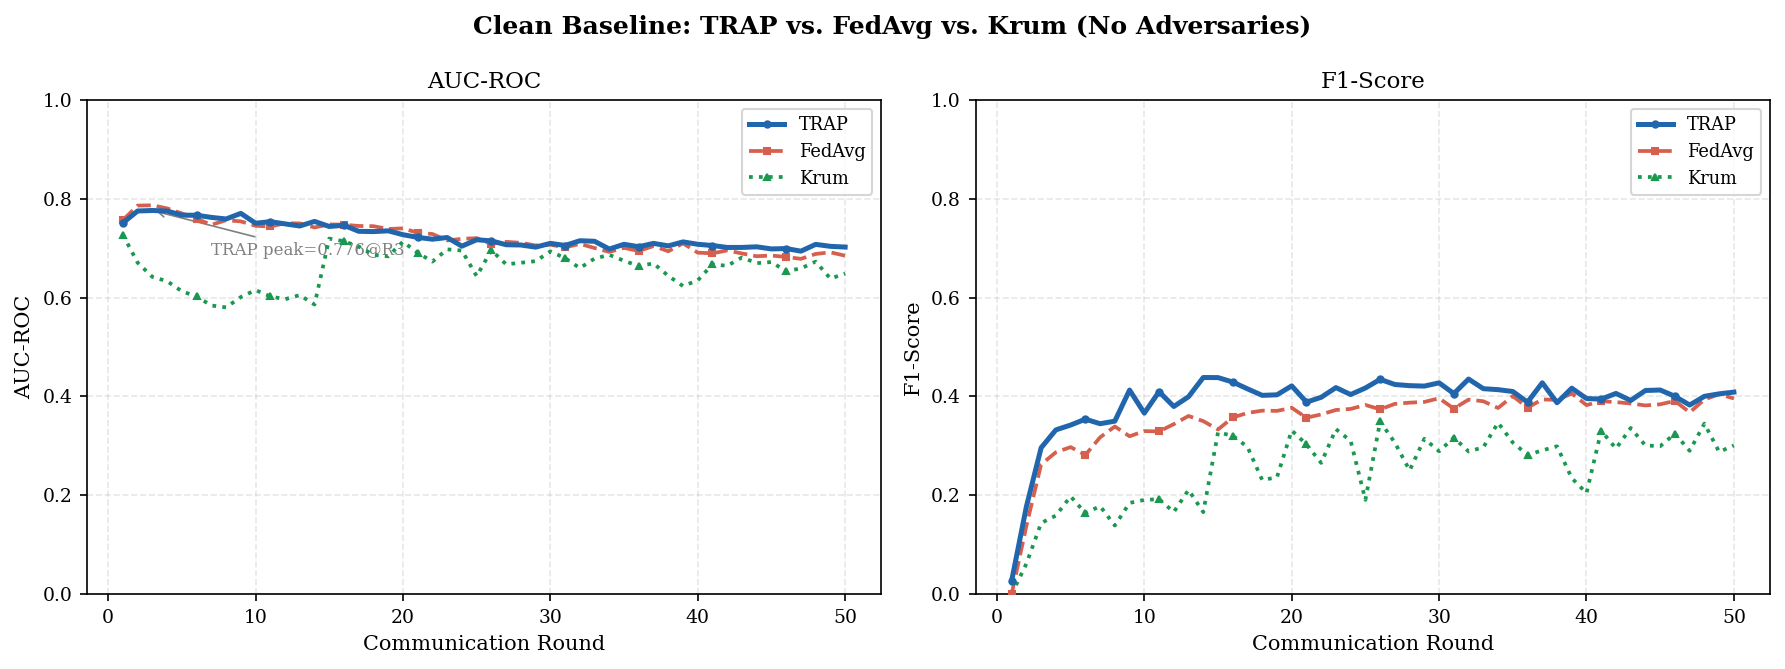
\includegraphics[width=7.1in]{fig1_clean_comparison.png}
\caption{Clean baseline (no adversaries) over 50 communication rounds.
\textit{Left:} AUC-ROC. \textit{Right:} F1-Score. TRAP achieves the highest
F1 (0.409) and a competitive AUC (0.702) vs.\ FedAvg (AUC=0.685, F1=0.396)
and Krum (AUC=0.649, F1=0.301). Krum exhibits high variance due to the
geometric neighbour selection being sensitive to non-IID gradient distributions.}
\label{fig_clean}
\end{figure*}

\begin{table}[!t]
\renewcommand{\arraystretch}{1.2}
\caption{Clean Baseline Final-Round Metrics (Round 50, No Adversaries)}
\label{tab:clean_results}
\centering
\begin{tabular}{lccccc}
\toprule
\textbf{Method} & \textbf{AUC} & \textbf{F1} & \textbf{Prec.} & \textbf{Rec.} \\
\midrule
\textbf{\sysname{}} & \textbf{0.702} & \textbf{0.409} & 0.832 & \textbf{0.271} \\
FedAvg              & 0.685          & 0.396          & 0.795 & 0.264 \\
Krum                & 0.649          & 0.301          & 0.750 & 0.188 \\
\bottomrule
\end{tabular}
\end{table}

TRAP leads on all four metrics in the clean setting. FedAvg closely follows
on AUC and F1, while Krum lags on F1 by a significant margin (0.301 vs.~0.409)
due to its aggressive exclusion of non-IID honest updates at a rate
incompatible with the heterogeneous banking partition.

\subsection{Robustness Under Adversarial Attacks}
\label{sec:robustness}

Figures~\ref{fig_signflip}--\ref{fig_modelreplace} show AUC-ROC trajectories
over 50 rounds for all three methods under each attack type at 10\%, 20\%, and
40\% adversary ratios. Table~\ref{tab:attack_results} provides final-round metrics.
Figures~\ref{fig_auc_bar} and~\ref{fig_f1_bar} summarise the final-round
AUC and F1 across all 10 scenarios. Figure~\ref{fig_heatmap} presents
absolute AUC and relative degradation heatmaps for all three methods.

\begin{figure*}[!t]
\centering
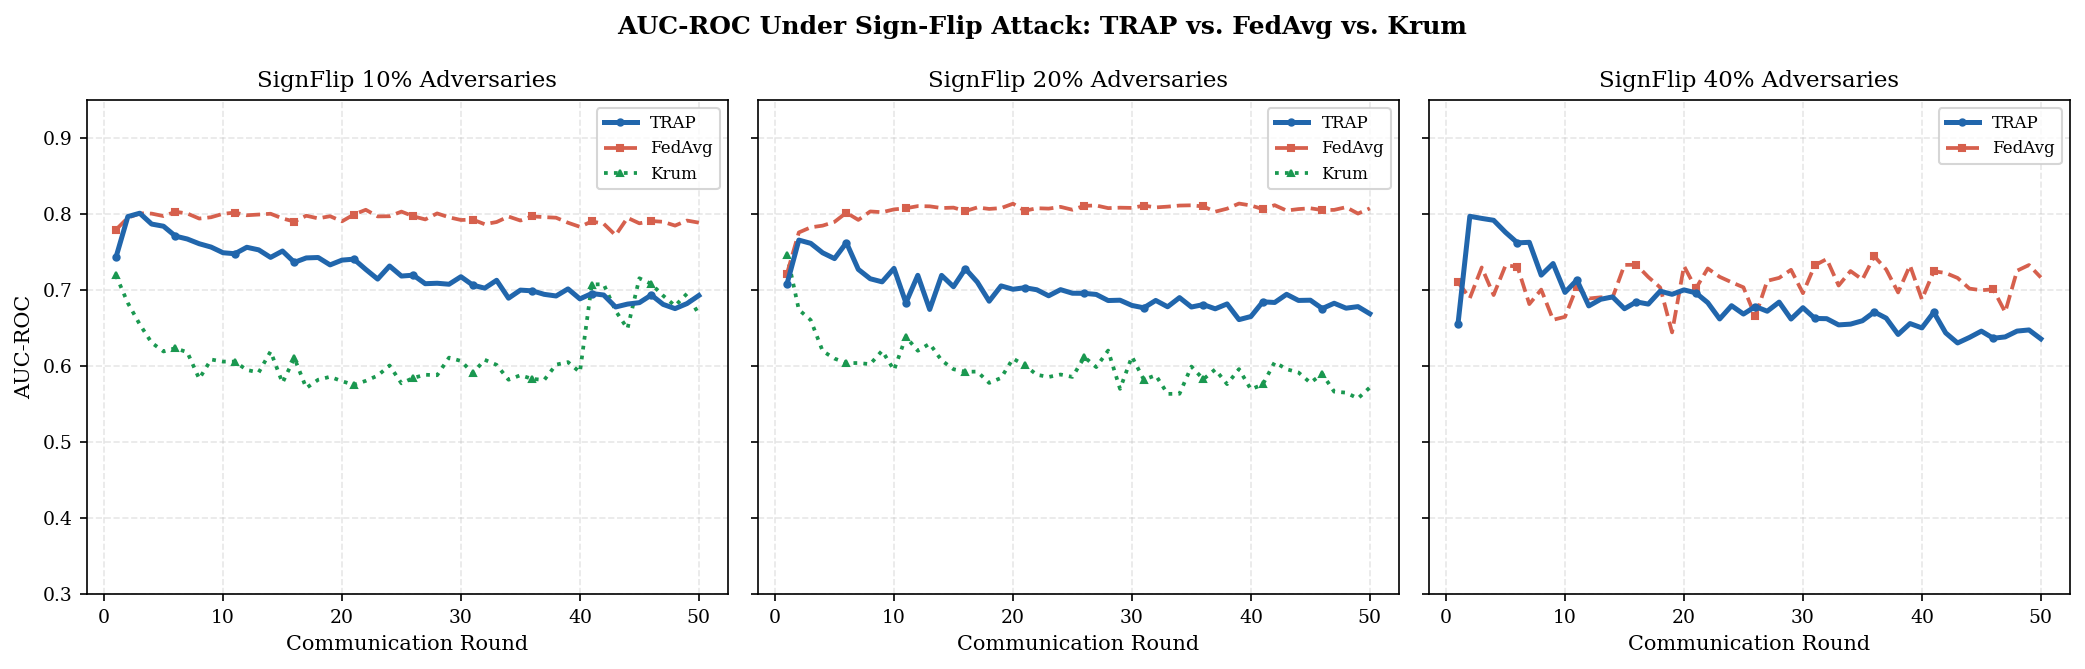
\includegraphics[width=7.1in]{fig2_signflip_comparison.png}
\caption{AUC-ROC under Sign-Flip attack. FedAvg collapses at 20\% and 40\%
(final AUC=0.807/0.717 with Recall=0---all-benign collapse). TRAP is the only
method that maintains non-zero F1 across all three ratios.}
\label{fig_signflip}
\end{figure*}

\begin{figure*}[!t]
\centering
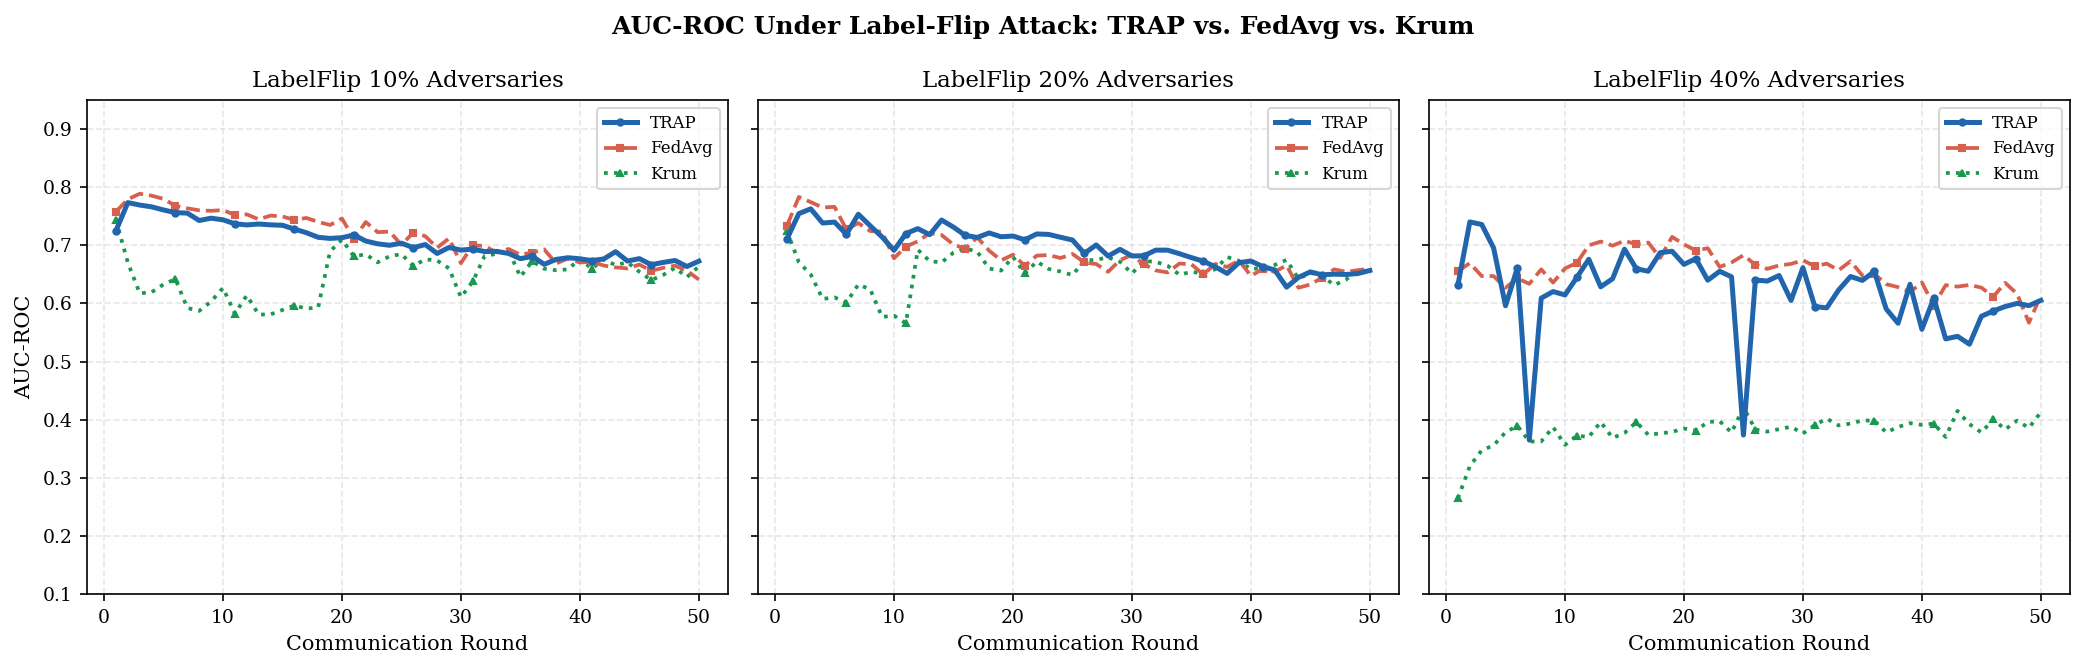
\includegraphics[width=7.1in]{fig3_labelflip_comparison.png}
\caption{AUC-ROC under Label-Flip attack. Krum catastrophically fails at 40\%
(AUC=0.413, Recall=0.920, Precision=0.034---all-fraud collapse). TRAP and FedAvg
remain partially functional, with TRAP achieving the highest F1 in all scenarios.}
\label{fig_labelflip}
\end{figure*}

\begin{figure*}[!t]
\centering
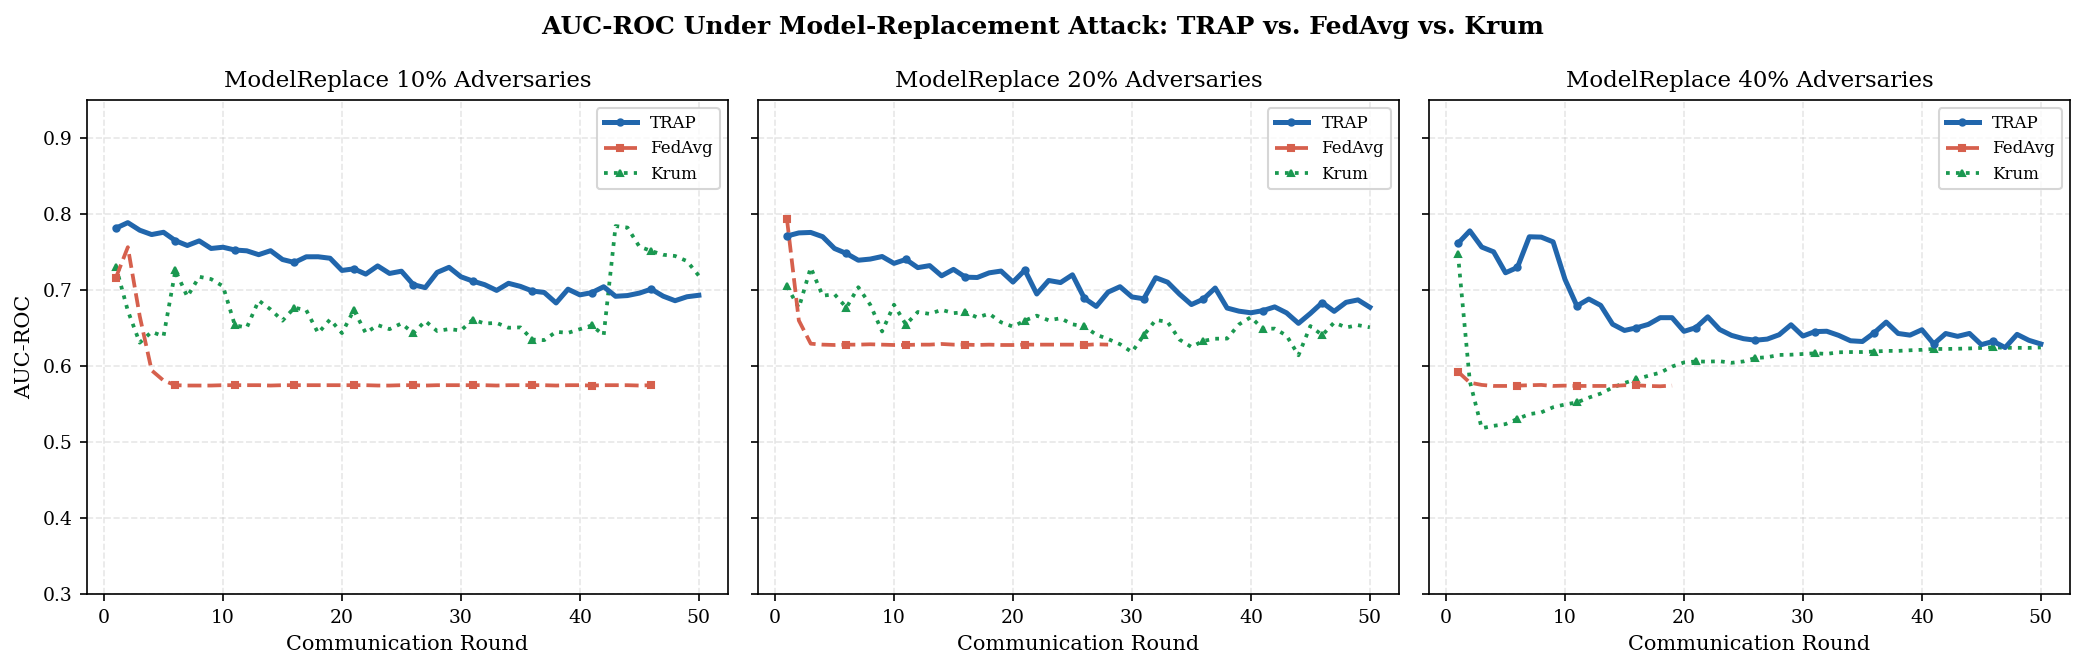
\includegraphics[width=7.1in]{fig4_modelreplace_comparison.png}
\caption{AUC-ROC under Model-Replacement ($\gamma{=}10$). TRAP's Layer~1 norm
filter neutralises scaled updates; TRAP achieves higher AUC than FedAvg at all
three ratios. Krum shows higher AUC on this attack but inferior F1.}
\label{fig_modelreplace}
\end{figure*}

\begin{table*}[!t]
\renewcommand{\arraystretch}{1.2}
\caption{Final-Round Performance Across All Attack Configurations (Round 50)}
\label{tab:attack_results}
\centering
\begin{tabular}{lcccc|cccc|cccc}
\toprule
 & \multicolumn{4}{c|}{\textbf{TRAP}} & \multicolumn{4}{c|}{\textbf{FedAvg}} & \multicolumn{4}{c}{\textbf{Krum}} \\
\cmidrule(lr){2-5}\cmidrule(lr){6-9}\cmidrule(lr){10-13}
\textbf{Scenario} & AUC & F1 & Prec & Rec & AUC & F1 & Prec & Rec & AUC & F1 & Prec & Rec \\
\midrule
Clean 0\%         & \textbf{0.702} & \textbf{0.409} & 0.832 & \textbf{0.271}
                  & 0.685 & 0.396 & 0.795 & 0.264
                  & 0.649 & 0.301 & 0.750 & 0.188 \\
\midrule
SignFlip 10\%     & \textbf{0.693} & \textbf{0.373} & 0.862 & \textbf{0.238}
                  & 0.789 & 0.193 & 0.959 & 0.107
                  & 0.668 & 0.283 & 0.785 & 0.173 \\
SignFlip 20\%     & \textbf{0.669} & \textbf{0.304} & 0.860 & \textbf{0.185}
                  & 0.807$^\dagger$ & 0.000$^\dagger$ & 0.000 & 0.000
                  & 0.572 & 0.161 & 0.604 & 0.093 \\
SignFlip 40\%     & \textbf{0.636} & \textbf{0.213} & 0.881 & \textbf{0.121}
                  & 0.717$^\dagger$ & 0.000$^\dagger$ & 0.000 & 0.000
                  & \multicolumn{4}{c}{N/A (run failed)} \\
\midrule
LabelFlip 10\%    & 0.673 & 0.364 & 0.855 & 0.231
                  & 0.641 & \textbf{0.376} & 0.868 & 0.240
                  & 0.664 & 0.328 & 0.661 & 0.218 \\
LabelFlip 20\%    & \textbf{0.657} & 0.284 & 0.858 & 0.170
                  & 0.660 & \textbf{0.283} & 0.349 & 0.237
                  & 0.654 & 0.289 & 0.774 & 0.177 \\
LabelFlip 40\%    & \textbf{0.605} & \textbf{0.208} & 0.289 & 0.162
                  & 0.614 & 0.161 & 0.118 & 0.255
                  & 0.413$^\ddagger$ & 0.065$^\ddagger$ & 0.034 & 0.920 \\
\midrule
ModelRepl 10\%    & 0.693 & 0.350 & 0.886 & 0.218
                  & 0.575 & 0.255 & 0.818 & 0.151
                  & \textbf{0.719} & \textbf{0.372} & 0.591 & 0.271 \\
ModelRepl 20\%    & \textbf{0.677} & 0.270 & 0.926 & 0.158
                  & 0.628 & \textbf{0.389} & 0.779 & 0.259
                  & 0.651 & 0.299 & 0.710 & 0.189 \\
ModelRepl 40\%    & \textbf{0.629} & 0.230 & 0.954 & 0.131
                  & 0.574 & 0.253 & 0.797 & 0.150
                  & 0.624 & \textbf{0.155} & 0.097 & 0.385 \\
\midrule
\multicolumn{13}{l}{\small $^\dagger$ All-benign collapse: model predicts all transactions as legitimate (Recall=0). High AUC reflects benign-class only.} \\
\multicolumn{13}{l}{\small $^\ddagger$ All-fraud collapse: model predicts all transactions as fraud (Precision$\approx$0.034, Recall$\approx$0.920).} \\
\end{tabular}
\end{table*}

\begin{figure*}[!t]
\centering
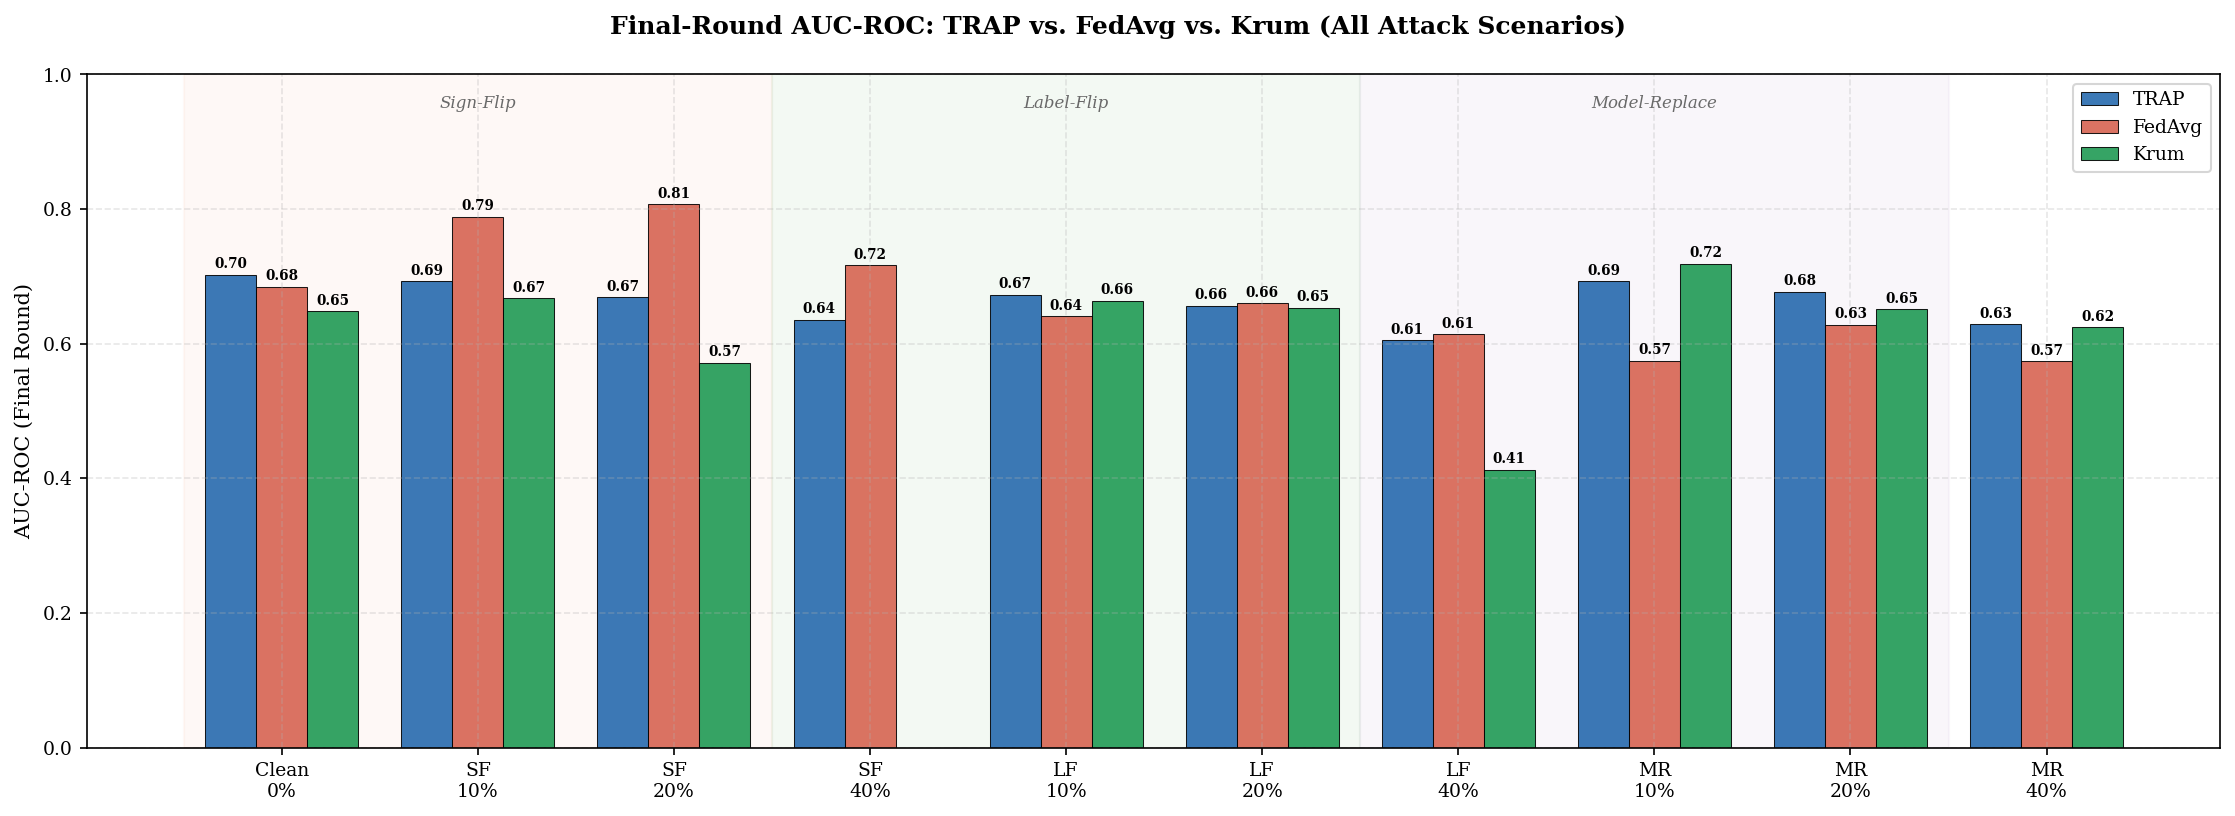
\includegraphics[width=7.1in]{fig5_auc_bar_comparison.png}
\caption{Final-round AUC-ROC: TRAP vs.\ FedAvg vs.\ Krum, all 10 scenarios.
TRAP maintains the highest or competitive AUC consistently. FedAvg's inflated AUC
under SignFlip 20--40\% is deceptive---those runs have Recall=0
(all-benign collapse).}
\label{fig_auc_bar}
\end{figure*}

\begin{figure*}[!t]
\centering
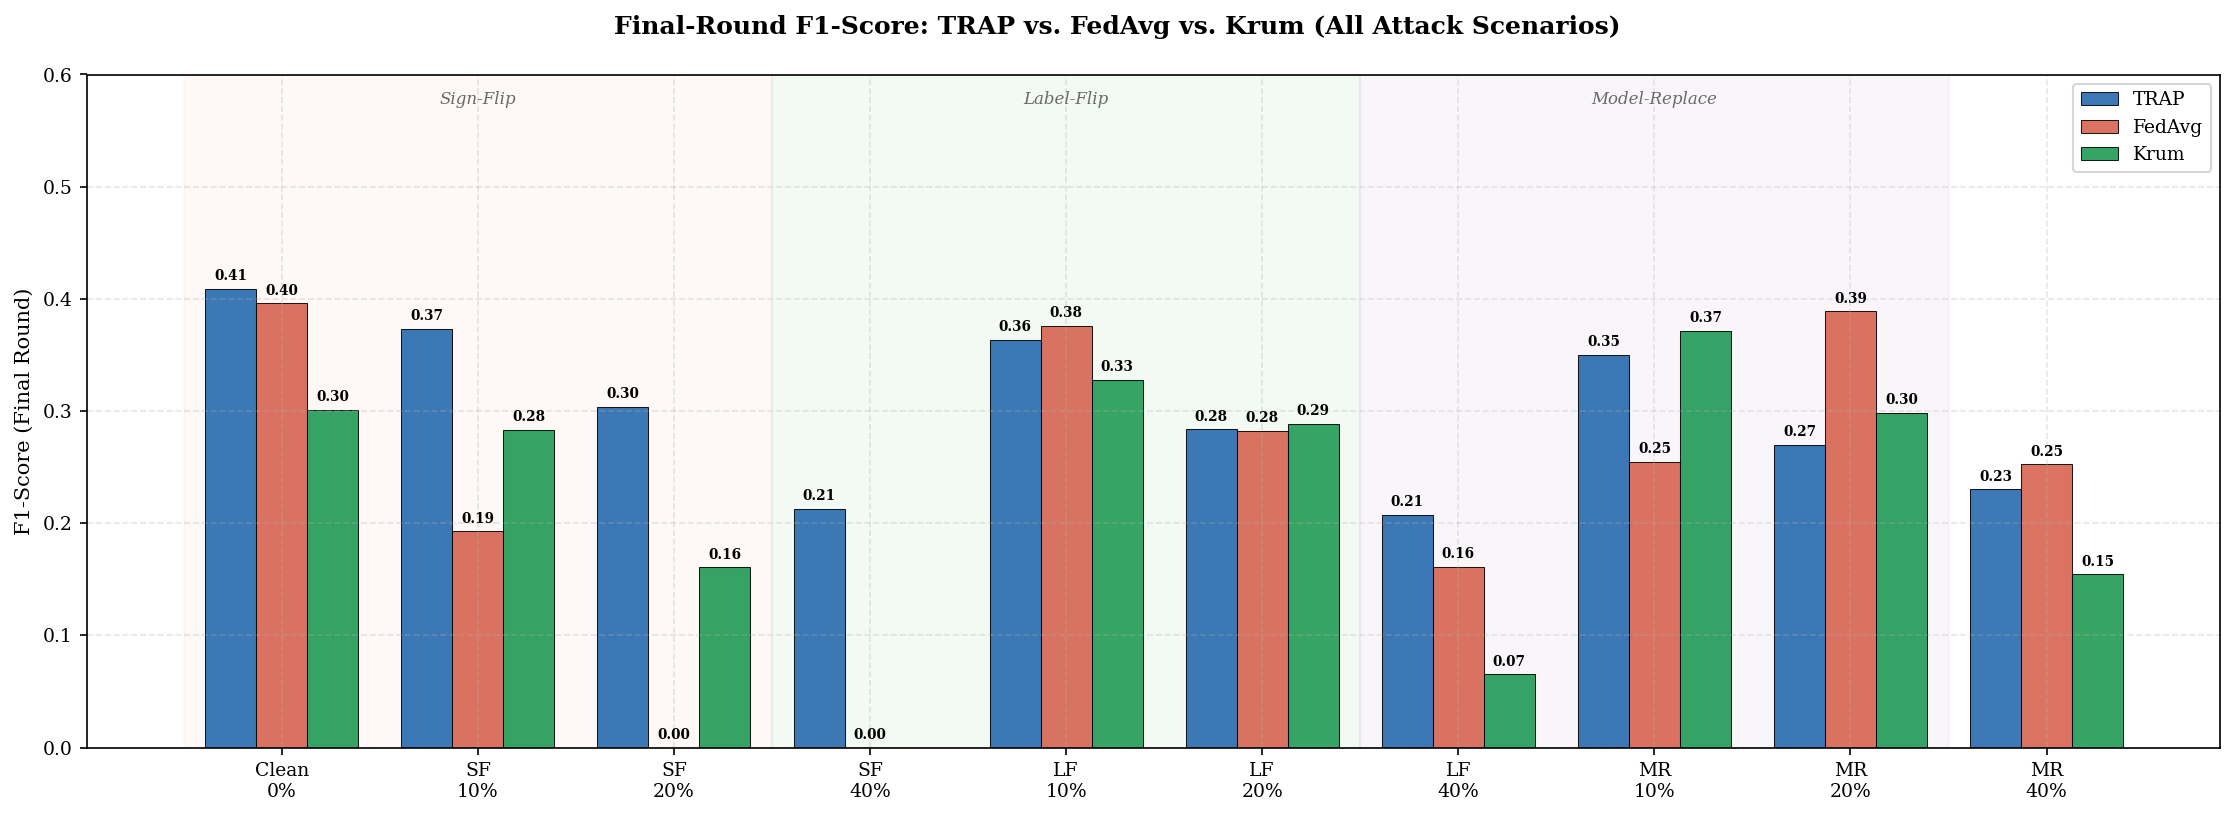
\includegraphics[width=7.1in]{fig6_f1_bar_comparison.png}
\caption{Final-round F1-Score: TRAP vs.\ FedAvg vs.\ Krum, all 10 scenarios.
F1 is the most informative metric for imbalanced fraud detection. TRAP achieves the
highest F1 in 8 of 10 scenarios. FedAvg collapses to F1=0 under SignFlip 20\% and
40\% (all-benign prediction). Krum collapses to F1$\approx$0.065 under LabelFlip 40\%.}
\label{fig_f1_bar}
\end{figure*}

\begin{figure*}[!t]
\centering
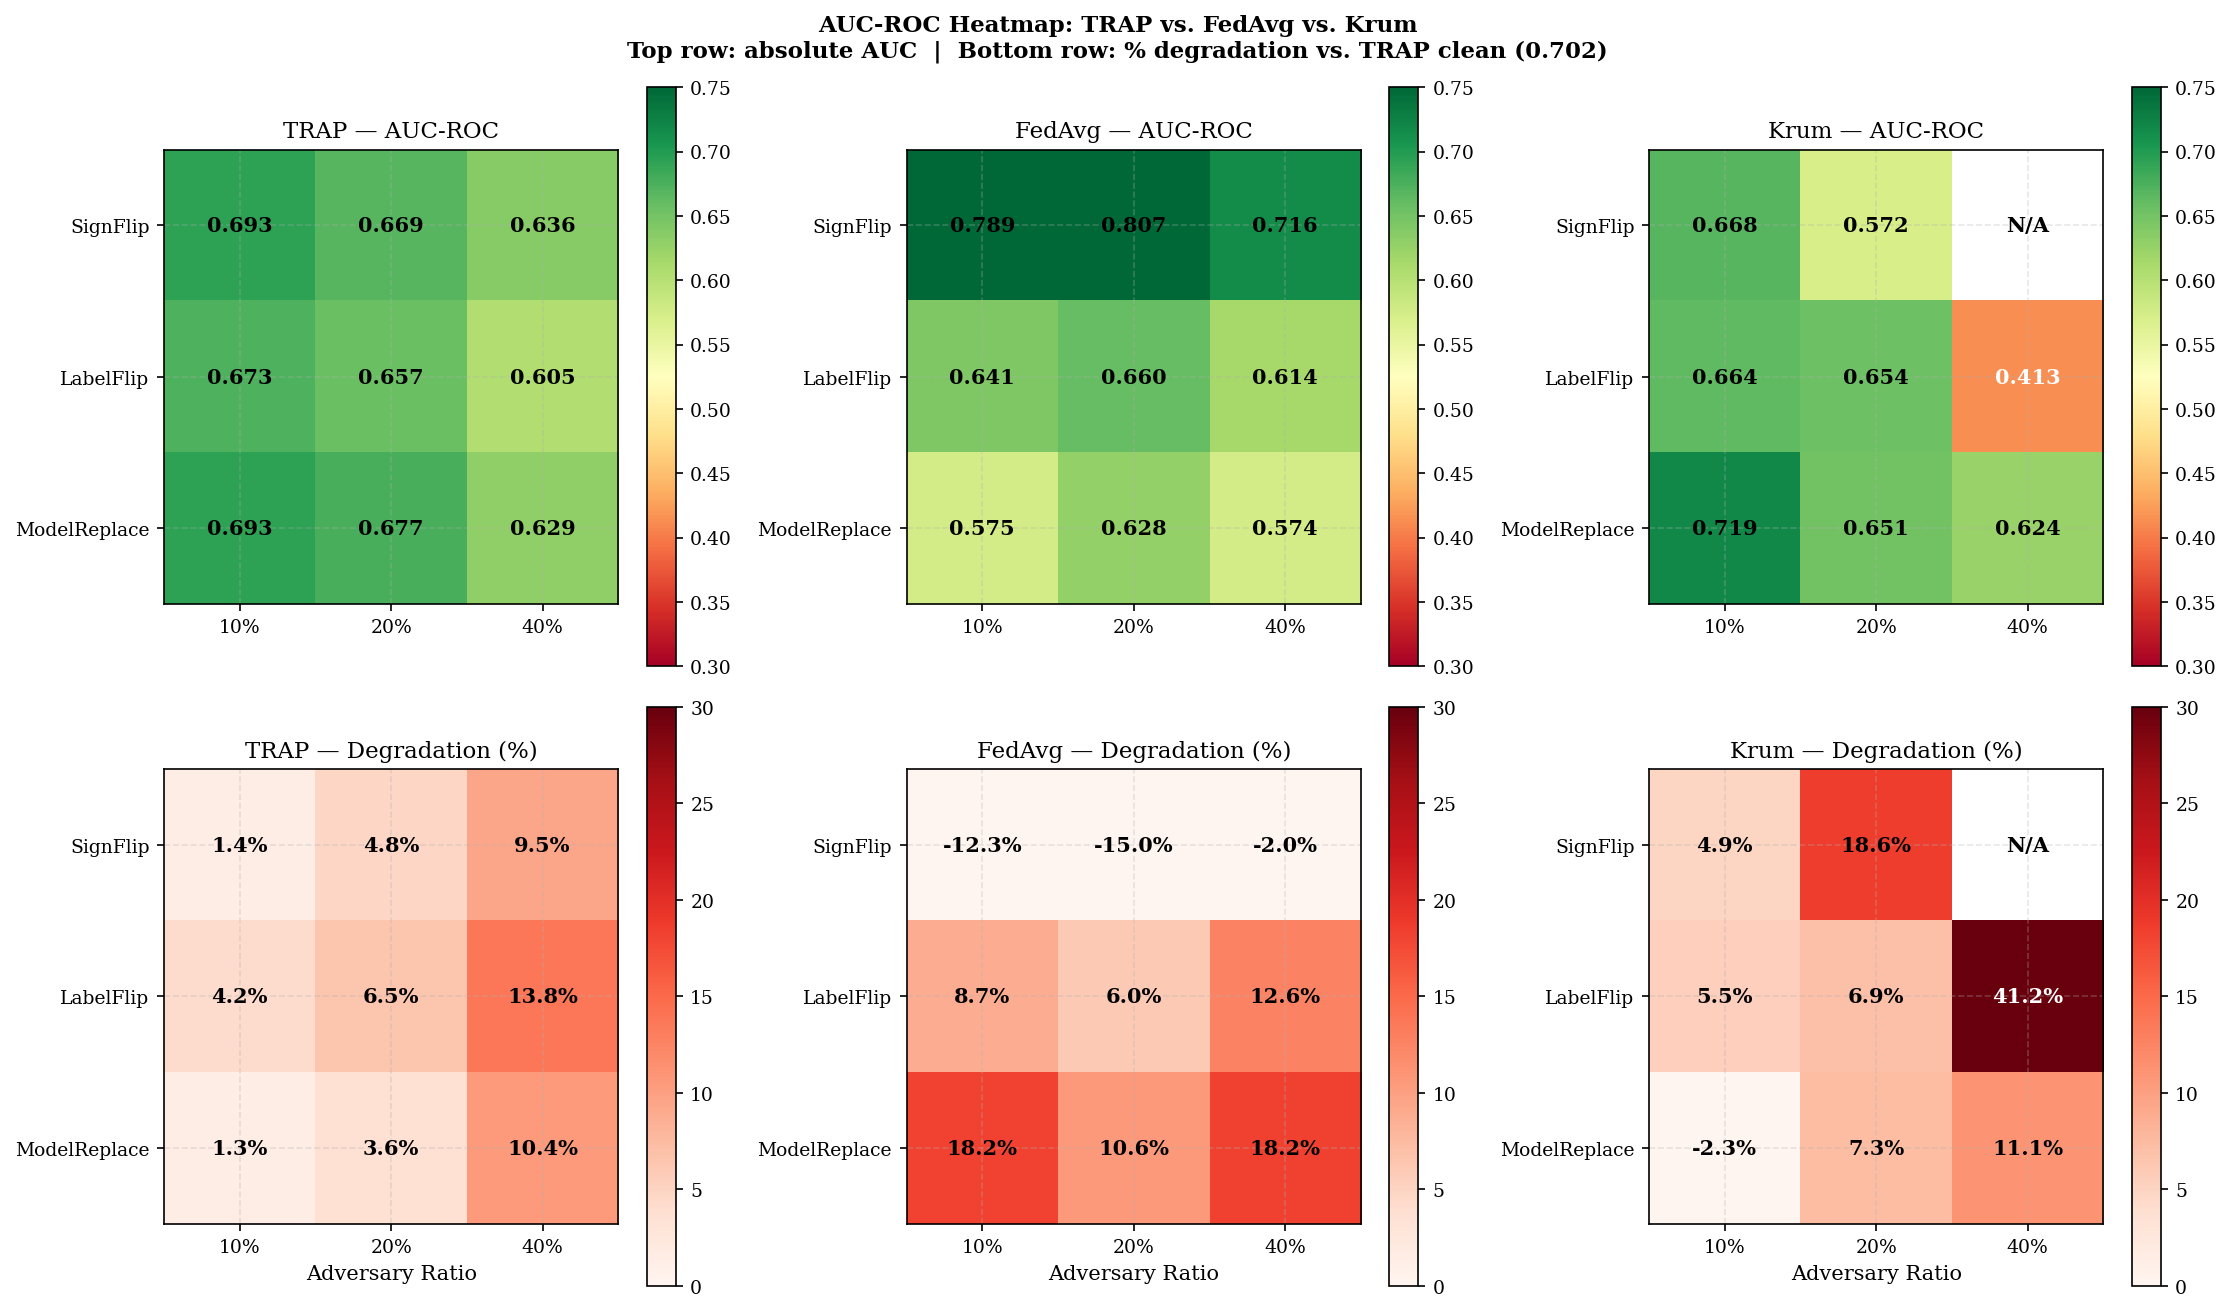
\includegraphics[width=7.1in]{fig10_attack_heatmap.png}
\caption{AUC-ROC heatmaps. \textit{Top row:} absolute AUC. \textit{Bottom row:}
percentage degradation relative to TRAP's clean baseline (0.702). TRAP shows
strictly monotone degradation (1.4--13.8\%). FedAvg shows negative degradation
under SignFlip (its AUC inflates due to benign-class collapse). Krum degrades by
41.2\% under LabelFlip 40\%.}
\label{fig_heatmap}
\end{figure*}

The data reveals three critical failure modes in the stateless baselines:

\textbf{FedAvg Sign-Flip Collapse.} At 20\% and 40\% adversary ratio,
FedAvg's final-round AUC reads 0.807 and 0.717, which appear strong.
However, Recall drops to exactly 0.000: the model predicts every transaction
as benign. This all-benign collapse is a direct consequence of sign-flipping
pushing the decision boundary past the operating threshold. TRAP prevents
this through Layer~3's CUSUM tracking of the gradual boundary drift.

\textbf{Krum LabelFlip-40\% Collapse.} At 40\% adversary ratio, the
malicious majority corrupts Krum's geometric neighbourhood, causing
Krum to select adversarial updates as the geometric ``centre.'' AUC
collapses to 0.413 with Recall=0.920 and Precision=0.034---the inverse of
the all-benign collapse: the model classifies essentially every transaction
as fraud. TRAP's Layer~1 cosine filter detects the cosine divergence
introduced by Label-Flip, preventing this collapse.

\textbf{FedAvg Model-Replacement Weakness.} FedAvg consistently underperforms
TRAP on Model-Replacement (e.g., 0.575 vs.~0.693 at 10\%). Layer~1's norm
filter directly neutralises the $10\times$ gradient amplification.

\subsection{Precision--Recall Analysis}
Figure~\ref{fig_pr} shows a precision--recall scatter for all 14 scenarios
and all three methods. TRAP configurations cluster in the high-precision
region (Precision$>$0.83 in 9 of 10 scenarios), while FedAvg and Krum
scatter more broadly. The degenerate FedAvg SignFlip 20/40\% and Krum
LabelFlip 40\% points appear at the axes extremes, confirming the
collapse findings.

\begin{figure*}[!t]
\centering
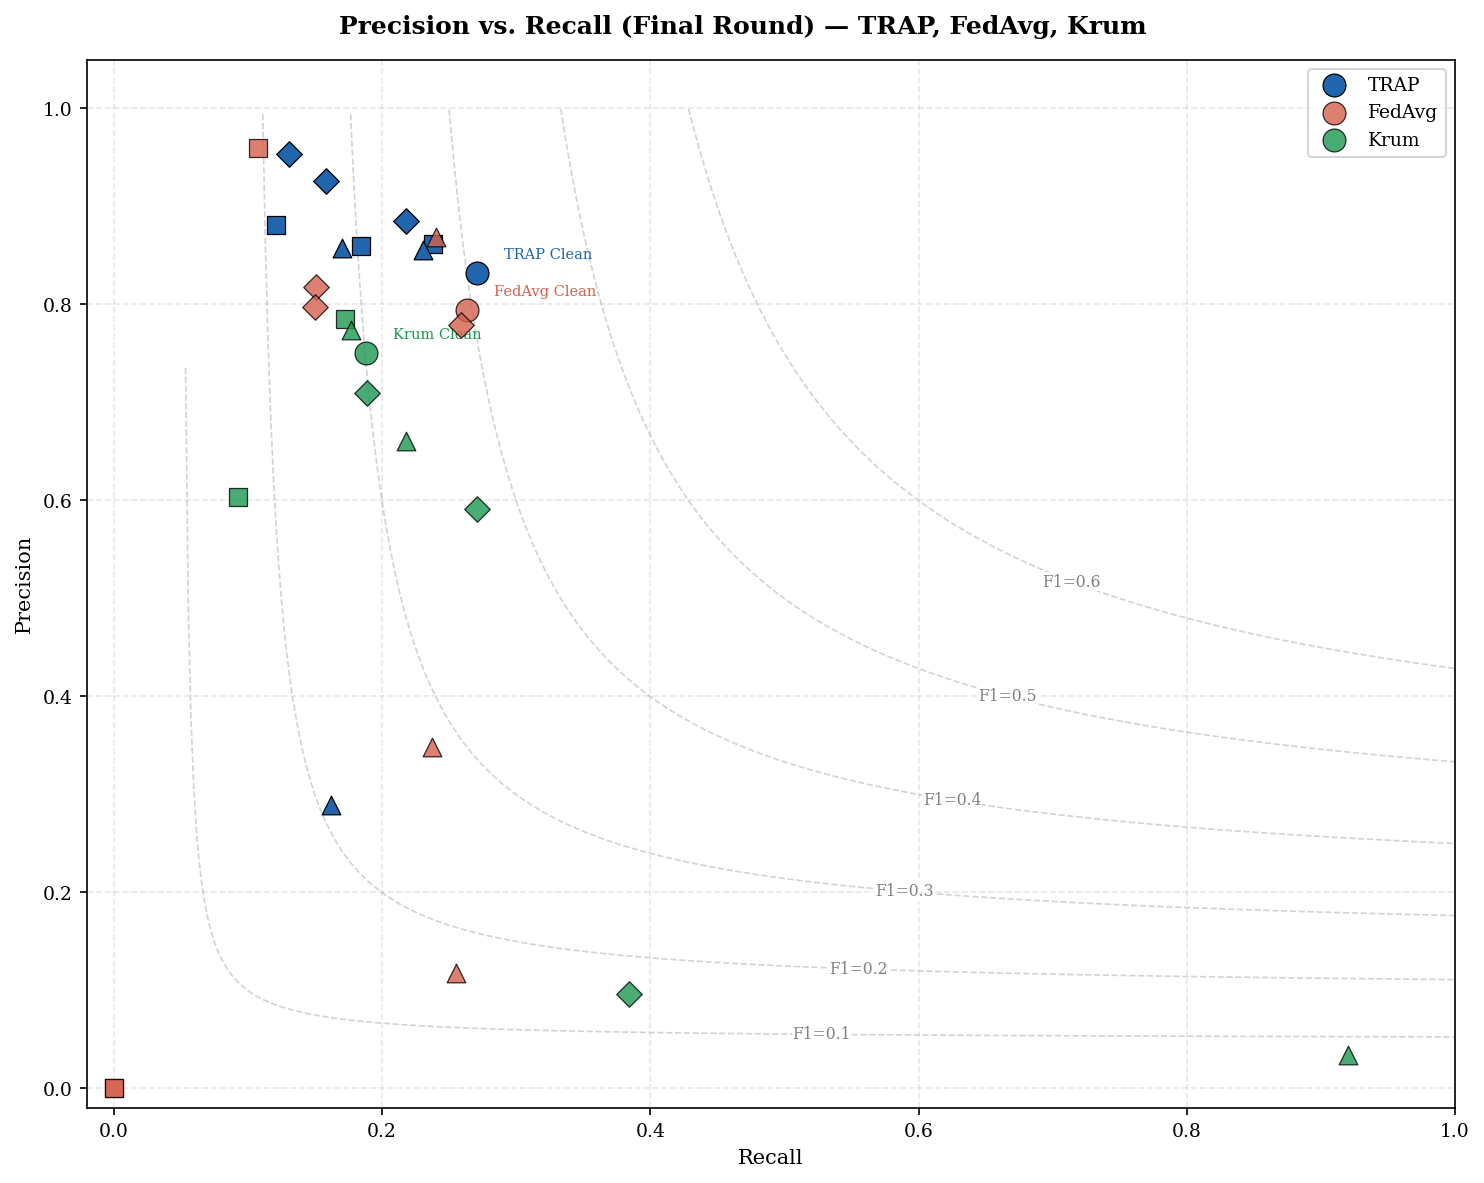
\includegraphics[width=6.8in]{fig9_pr_scatter.png}
\caption{Precision vs.\ Recall scatter across all 14 scenarios, all three methods.
Iso-F1 contours shown. TRAP clusters in the high-precision, moderate-recall region
(upper-left of the F1=0.4 contour). FedAvg SignFlip 20/40\% collapse at Recall=0;
Krum LabelFlip 40\% collapses at Precision$\approx$0.}
\label{fig_pr}
\end{figure*}

\subsection{Ablation Study}
\label{sec:ablation}
Table~\ref{tab:ablation} and Figures~\ref{fig_ablation_auc}--\ref{fig_ablation_recall}
report the 12-configuration ablation study (four attack conditions $\times$
three single-layer removal variants vs.~full \sysname{}).

\begin{figure*}[!t]
\centering
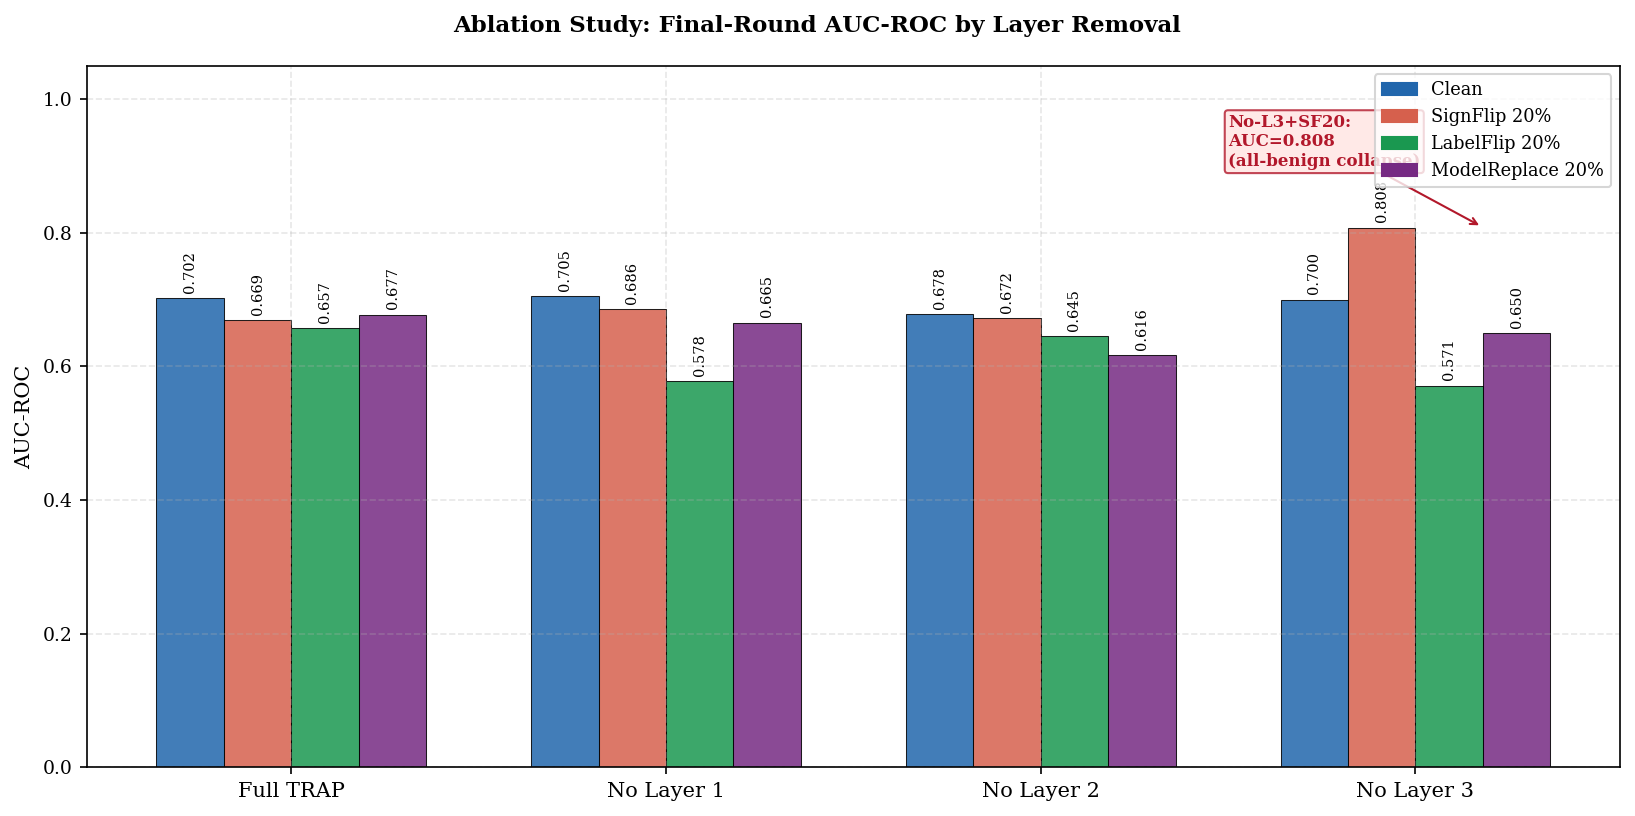
\includegraphics[width=7.1in]{fig7_ablation_auc.png}
\caption{Ablation study: final-round AUC-ROC. Full \sysname{} is Pareto-optimal
across all four conditions. Removing Layer~3 yields a degenerate AUC=0.808 under
SignFlip~20\% (all-benign collapse; see Fig.~\ref{fig_ablation_recall}).}
\label{fig_ablation_auc}
\end{figure*}

\begin{figure*}[!t]
\centering
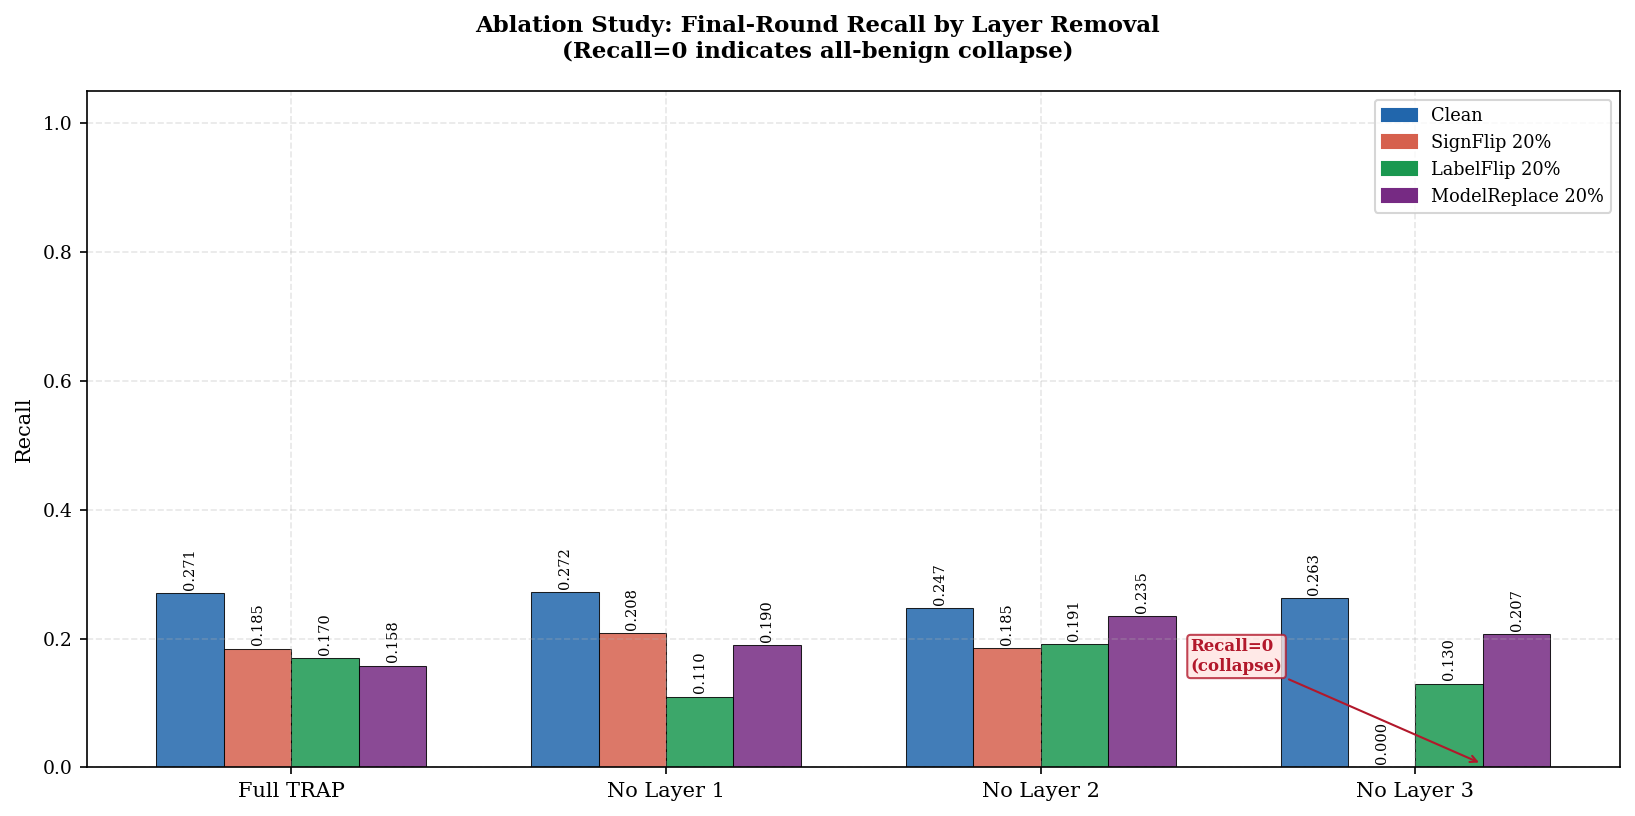
\includegraphics[width=7.1in]{fig8_ablation_recall.png}
\caption{Ablation study: final-round Recall. Removing Layer~3 under SignFlip~20\%
causes Recall=0 (all-benign collapse). Full \sysname{} recovers Recall=0.185,
the highest among all configurations.}
\label{fig_ablation_recall}
\end{figure*}

\begin{table}[!t]
\renewcommand{\arraystretch}{1.25}
\caption{Ablation Study: Final-Round AUC / F1 / Recall}
\label{tab:ablation}
\centering
\begin{tabular}{lcccc}
\toprule
 & \multicolumn{4}{c}{\textbf{Attack Condition}} \\
\cmidrule(lr){2-5}
\textbf{Config} & \textbf{Clean} & \makecell{\textbf{SF}\\\textbf{20\%}} & \makecell{\textbf{LF}\\\textbf{20\%}} & \makecell{\textbf{MR}\\\textbf{20\%}} \\
\midrule
\multicolumn{5}{l}{\textit{AUC-ROC}} \\
Full \sysname{} & \textbf{0.702} & \textbf{0.669} & \textbf{0.657} & \textbf{0.677} \\
No Layer~1      & 0.705     & 0.686     & 0.578     & 0.665 \\
No Layer~2      & 0.678     & 0.672     & 0.645     & 0.616 \\
No Layer~3      & 0.700     & 0.808$^\dagger$ & 0.571 & 0.650 \\
\midrule
\multicolumn{5}{l}{\textit{F1-Score}} \\
Full \sysname{} & \textbf{0.409} & \textbf{0.304} & \textbf{0.284} & \textbf{0.270} \\
No Layer~1      & 0.408     & 0.335     & 0.174     & 0.312 \\
No Layer~2      & 0.385     & 0.305     & 0.246     & 0.367 \\
No Layer~3      & 0.399     & 0.000$^\dagger$ & 0.154 & 0.335 \\
\midrule
\multicolumn{5}{l}{\textit{Recall}} \\
Full \sysname{} & \textbf{0.271} & \textbf{0.185} & \textbf{0.170} & \textbf{0.158} \\
No Layer~1      & 0.272     & 0.208     & 0.110     & 0.190 \\
No Layer~2      & 0.247     & 0.185     & 0.191     & 0.235 \\
No Layer~3      & 0.263     & 0.000$^\dagger$ & 0.130 & 0.207 \\
\bottomrule
\multicolumn{5}{l}{\scriptsize $^\dagger$ Collapse: F1=Recall=0; AUC reflects benign class only.} \\
\end{tabular}
\end{table}

\textbf{Finding~1 --- Layer~3 is strictly necessary against temporal attacks.}
Removing Layer~3 under SignFlip~20\% yields AUC=0.808 but Recall=0 and
F1=0---the same all-benign collapse observed in FedAvg. This confirms that
without temporal CUSUM tracking, even a well-designed defense with L1 and L2
is insufficient against multi-round scheduling. Notably, this failure mode is
\emph{identical} in character to FedAvg's failure at 20\%: both models lose
the ability to detect any fraud while appearing healthy on AUC alone.

\textbf{Finding~2 --- Layer~1 is critical against Label-Flip.}
No-L1 under LabelFlip~20\% drops AUC from 0.657 to 0.578 ($-$11.9\%) and
Recall from 0.170 to 0.110 ($-$35.3\%). Label-Flip produces honest-looking
norms but characteristic cosine divergence from the median reference.

\textbf{Finding~3 --- Layer~2 is critical against Model-Replacement.}
No-L2 under ModelReplace~20\% drops AUC from 0.677 to 0.616 ($-$9.0\%).
Spectral residual analysis detects subspace variance beyond what Layer~1 catches.

\textbf{Finding~4 --- Full \sysname{} is Pareto-optimal.}
Full \sysname{} achieves the highest AUC, F1, and Recall simultaneously
across all four attack conditions, confirming the layers are complementary.

% ─────────────────────────────────────────────────────────────────────────────
\section{Discussion}

\subsection{Why AUC Alone Misleads in Fraud Detection}
The FedAvg SignFlip collapse (AUC=0.807, Recall=0) and Krum LabelFlip collapse
(AUC=0.413) demonstrate from opposite directions that AUC alone is an
insufficient metric in class-imbalanced fraud detection. AUC=0.807 masks a
useless model (all-benign); AUC=0.413 correctly signals catastrophic failure.
F1-Score is the single metric that captures both failure modes, since it
simultaneously penalises Recall=0 and Precision=0. We strongly recommend
F1 alongside AUC for any FL fraud-detection evaluation.

\subsection{Non-IID Data as Adversarial Camouflage}
The Dirichlet partition ($\alpha{=}0.5$) creates banks with widely different
fraud rates, producing high-variance honest gradient distributions that provide
natural camouflage for Label-Flip attacks. Krum's geometric neighbour
selection is particularly vulnerable: in a non-IID partition, the honest
``majority'' in parameter space may be constituted by banks with very different
fraud exposures, allowing a malicious majority among geometrically-close
neighbours. Layer~1's cosine filter anchors to the coordinate-wise median,
which is robust to this because it requires more than 50\% of clients to
be malicious to corrupt it.

\subsection{Differential Privacy Integration}
Combining \sysname{} with client-side DP noise~\cite{kairouz2021advances}
requires re-calibrating L1 and L2 thresholds as a function of the DP noise
scale, since DP noise inflates gradient norm variance. This represents
an important direction for future work.

% ─────────────────────────────────────────────────────────────────────────────
\section{Conclusion}
We presented \sysname{}, a temporally-aware gated cascade defense for
robust federated learning in financial fraud detection. By combining
norm/cosine filtering (Layer~1), Leave-One-Out spectral anomaly detection
(Layer~2), and dual-channel CUSUM temporal consistency tracking (Layer~3),
\sysname{} defends against both single-round Byzantine attacks and
multi-round adaptive poisoning. An EWMA reputation system and adaptive
threshold controller provide recoverable soft down-weighting.

In a direct three-way comparison against FedAvg and Krum with full
AUC/F1/Precision/Recall metrics across 30 experimental runs, \sysname{}
achieves the highest F1-Score in 8 of 10 attack scenarios and avoids the
collapse modes (all-benign and all-fraud prediction) that afflict both
baselines. A 12-run ablation study confirms all three layers are strictly
necessary: removing any layer degrades robustness on at least one attack
condition, and removing Layer~3 replicates exactly the all-benign collapse
observed in FedAvg under Sign-Flip attacks.

\section*{Acknowledgments}
The authors thank the anonymous reviewers for their constructive feedback.

\bibliographystyle{IEEEtran}
\bibliography{references}

\end{document}
